\section{NVIDIA 历史}

在上个世纪的最后二十年里，几家如今众所周知的巨头公司相继成立，其中最伟大之一就是英伟达（NVIDIA）。英伟达由黄仁勋于
1993 年创立。成立仅两年后，英伟达推出了其第一款产品——NV1。该设备设计相当简单，其 GPU 仅有 2 MB 内存、64 位总线
宽度和单个核心。要了解如今的差距，可以将其与最新的 GPU GeForce RTX 4090 Ti 进行比较：RTX 4090 Ti 拥有约 18,000
个核心，而 NV1 只有 1 个核心。


\begin{figure}
    \centering
    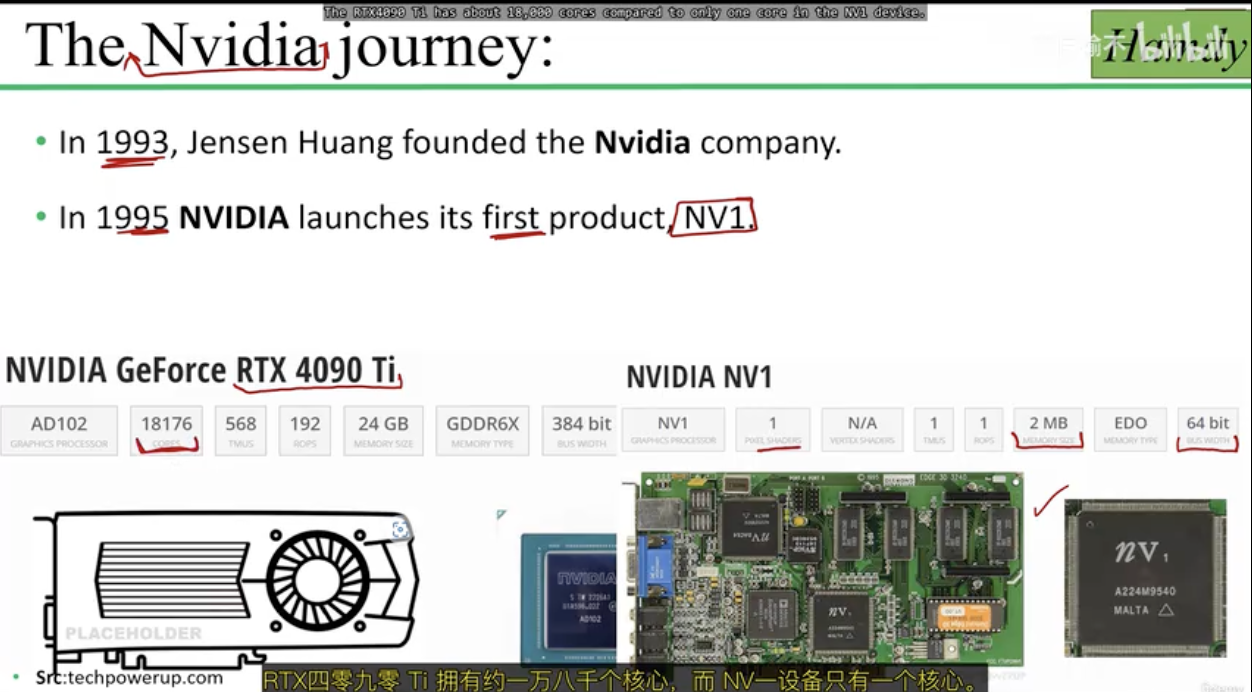
\includegraphics[width=0.75\linewidth]{resources/cuda-007.png}
    \caption{NVIDIA 历史}
    \label{fig:placeholder}
\end{figure}

核心数量方面，增长了约 18,000 倍。而内存容量从 NV1 的 2 MB 增加到 RTX 4090 Ti 的 48 GB，增长约 24,000 倍。此
外，再看看对应用程序性能至关重要的运行频率——已从 75 MHz 大幅提升至约 2400 MHz，带来 32 倍的速度提升。这充分展示了
GPU 技术在过去 25 年间的巨大演变。

\subsection{RIVA 128}

暂时放下这些数据，我们继续往下看。1997 年，英伟达推出了 RIVA 128，也称为 NV3。该型号是首批为消费级市场带来三维加速的
GPU 之一，这也是为什么它比其前身 NV1 更成功。值得注意的是，RIVA 128 是英伟达首次取得重大市场成功的产品，在巩固其市场
地位方面发挥了关键作用——四个月内销量即达到约 100 万台。

\begin{figure}
    \centering
    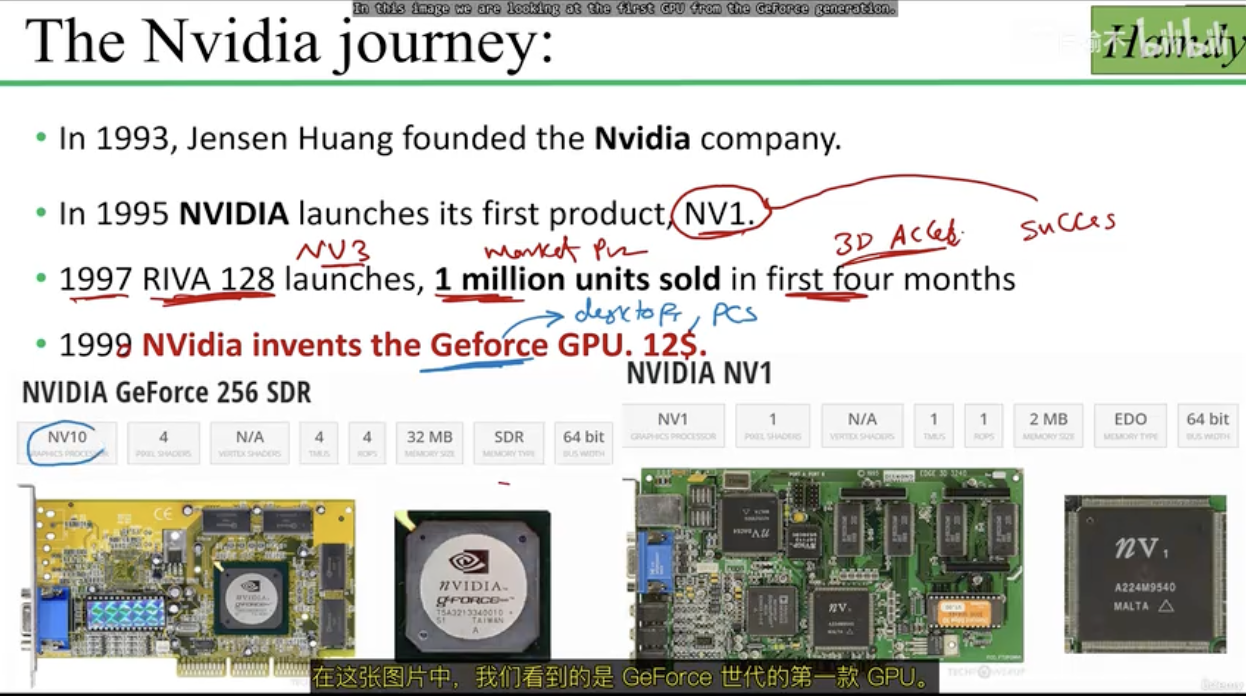
\includegraphics[width=0.75\linewidth]{resources/cuda-008.png}
    \caption{GeForce}
    \label{fig:placeholder}
\end{figure}

\subsection{GeForce世代}

GeForce 这一品牌为许多人所熟悉，因为这些 GPU 在问世一两年后就广泛出现在台式机和笔记本电脑中。具体来说，1998 年英伟达
揭开了后来成为其标志性 GPU 世代的 GeForce 系列的序幕。此次发布标志着 GPU 技术领域的一次革命性转变。从图中可以看到，
GeForce 系列的首款 GPU 与 NV1 相比差异巨大——它拥有四个核心，相对于英伟达第一款 GPU NV1 的单核心来说是一个巨大的飞
跃。别忘了，那是在 1998 年，一台设备中有四个核心本身就是一场革命。内存容量也从 NV1 的 2 MB 增加到 32 MB，增长了 16 倍。

从那时起，英伟达就成为全球 GPU 领域最知名的公司。如今，英伟达既是推动计算加速的关键力量，也主导着游戏产业。以上便是英伟
达发展历程的简要概述。
